\chapter{Flows and cuts}

In this chapter, we will focus on the following
problems in a directed, weighted graph
where a starting node and a ending node is given:

\begin{itemize}
\item \key{Finding a maximum flow}:
What is the maximum amount of flow we can
deliver
from the starting node to the ending node?
\item \key{Finding a minimum cut}:
What is a minimum-weight set of edges
that separates the starting node and the ending node?
\end{itemize}

It turns out that these problems correspond to
each other, and we can solve them simultaneously
using the same algorithm.

As an example, we will use the following graph
where node 1 is the starting node and node 6
is the ending node:

\begin{center}
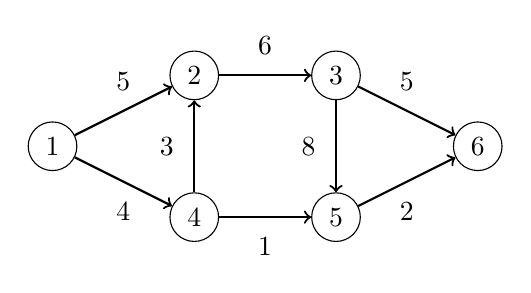
\begin{tikzpicture}[scale=0.9]
\node[draw, circle] (1) at (1,2) {$1$};
\node[draw, circle] (2) at (3,3) {$2$};
\node[draw, circle] (3) at (5,3) {$3$};
\node[draw, circle] (4) at (7,2) {$6$};
\node[draw, circle] (5) at (3,1) {$4$};
\node[draw, circle] (6) at (5,1) {$5$};
\path[draw,thick,->] (1) -- node[font=\small,label=5] {} (2);
\path[draw,thick,->] (2) -- node[font=\small,label=6] {} (3);
\path[draw,thick,->] (3) -- node[font=\small,label=5] {} (4);
\path[draw,thick,->] (1) -- node[font=\small,label=below:4] {} (5);
\path[draw,thick,->] (5) -- node[font=\small,label=below:1] {} (6);
\path[draw,thick,->] (6) -- node[font=\small,label=below:2] {} (4);
\path[draw,thick,<-] (2) -- node[font=\small,label=left:3] {} (5);
\path[draw,thick,->] (3) -- node[font=\small,label=left:8] {} (6);
\end{tikzpicture}
\end{center}

\subsubsection{Maximum flow}

\index{flow}
\index{maximum flow}

A \key{maximum flow} is a flow from the
starting node to the ending node whose
total amount is as large as possible.
The weight of each edge is a capacity that
determines the maximum amount of flow that
can go through the edge.
In all nodes, except for the starting node
and the ending node,
the amount of incoming and outgoing flow
must be the same.

A maximum flow for the example graph
is as follows:

\begin{center}
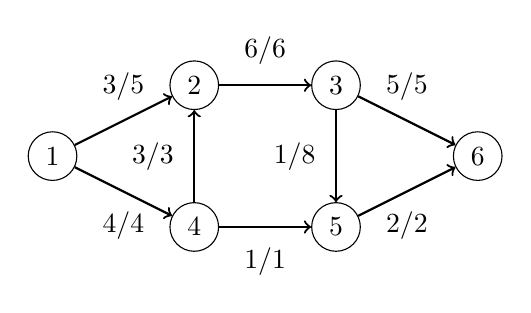
\begin{tikzpicture}[scale=0.9]
\node[draw, circle] (1) at (1,2) {$1$};
\node[draw, circle] (2) at (3,3) {$2$};
\node[draw, circle] (3) at (5,3) {$3$};
\node[draw, circle] (4) at (7,2) {$6$};
\node[draw, circle] (5) at (3,1) {$4$};
\node[draw, circle] (6) at (5,1) {$5$};
\path[draw,thick,->] (1) -- node[font=\small,label=3/5] {} (2);
\path[draw,thick,->] (2) -- node[font=\small,label=6/6] {} (3);
\path[draw,thick,->] (3) -- node[font=\small,label=5/5] {} (4);
\path[draw,thick,->] (1) -- node[font=\small,label=below:4/4] {} (5);
\path[draw,thick,->] (5) -- node[font=\small,label=below:1/1] {} (6);
\path[draw,thick,->] (6) -- node[font=\small,label=below:2/2] {} (4);
\path[draw,thick,<-] (2) -- node[font=\small,label=left:3/3] {} (5);
\path[draw,thick,->] (3) -- node[font=\small,label=left:1/8] {} (6);
\end{tikzpicture}
\end{center}

The notation $v/k$ means
that amount of the flow through the edge is $v$
and the capacity of the edge is $k$.
For each edge, it is required that $v \le k$.
In this graph, the size of a maximum flow is 7
because the outgoing flow from the starting node is $3+4=7$,
and the incoming flow to the ending node is $5+2=7$.

Note that in each intermediate node,
the incoming flow and the outgoing flow are equally large.
For example, in node 2, the incoming flow is $3+3=6$
from nodes 1 and 4,
and the outgoing flow is $6$ to node 3.

\subsubsection{Minimum cut}

\index{cut}
\index{minimum cut}

A \key{minimum cut} is a set of edges
whose removal separates the starting node from the ending node,
and whose total weight is as small as possible.
A cut divides the graph into two components,
one containing the starting node and the other
containing the ending node.

A minimum cut for the example graph is as follows:

\begin{center}
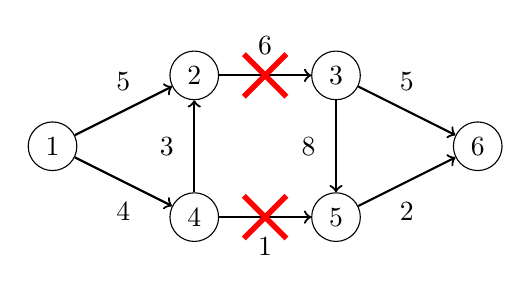
\begin{tikzpicture}[scale=0.9]
\node[draw, circle] (1) at (1,2) {$1$};
\node[draw, circle] (2) at (3,3) {$2$};
\node[draw, circle] (3) at (5,3) {$3$};
\node[draw, circle] (4) at (7,2) {$6$};
\node[draw, circle] (5) at (3,1) {$4$};
\node[draw, circle] (6) at (5,1) {$5$};
\path[draw,thick,->] (1) -- node[font=\small,label=5] {} (2);
\path[draw,thick,->] (2) -- node[font=\small,label=6] {} (3);
\path[draw,thick,->] (3) -- node[font=\small,label=5] {} (4);
\path[draw,thick,->] (1) -- node[font=\small,label=below:4] {} (5);
\path[draw,thick,->] (5) -- node[font=\small,label=below:1] {} (6);
\path[draw,thick,->] (6) -- node[font=\small,label=below:2] {} (4);
\path[draw,thick,<-] (2) -- node[font=\small,label=left:3] {} (5);
\path[draw,thick,->] (3) -- node[font=\small,label=left:8] {} (6);

\path[draw=red,thick,-,line width=2pt] (4-.3,3-.3) -- (4+.3,3+.3);
\path[draw=red,thick,-,line width=2pt] (4-.3,3+.3) -- (4+.3,3-.3);
\path[draw=red,thick,-,line width=2pt] (4-.3,1-.3) -- (4+.3,1+.3);
\path[draw=red,thick,-,line width=2pt] (4-.3,1+.3) -- (4+.3,1-.3);
\end{tikzpicture}
\end{center}

In this cut, the first component contains nodes $\{1,2,4\}$,
and the second component contains nodes $\{3,5,6\}$.
The weight of the cut is 7,
because it consists of edges
$2 \rightarrow 3$ and $4 \rightarrow 5$,
and the total weight of the edges is $6+1=7$.
\\\\
It is not a coincidence that
both the size of the maximum flow and 
the weight of the minimum cut is 7
in the example graph.
It turns out that a maximum flow and
a minimum cut are \emph{always} of equal size,
so the concepts are two sides of the same coin.

Next we will discuss the Ford–Fulkerson
algorithm that can be used for finding
a maximum flow and a minimum cut in a graph.
The algorithm also helps us to understand
\emph{why} they are equally large.

\section{Ford–Fulkerson algorithm}

\index{Ford–Fulkerson algorithm}

The \key{Ford–Fulkerson algorithm} finds
a maximum flow in a graph.
The algorithm begins with an empty flow,
and at each step finds a path in the graph
that generates more flow.
Finally, when the algorithm can't extend the flow
anymore, it terminates and a maximum flow has been found.

The algorithm uses a special representation
for the graph  where each original edge has a reverse
edge in another direction.
The weight of each edge indicates how much more flow
we could route through it.
Initially, the weight of each original edge
equals the capacity of the edge,
and the weight of each reverse edge is zero.

\begin{samepage}
The new representation for the example graph is as follows:

\begin{center}
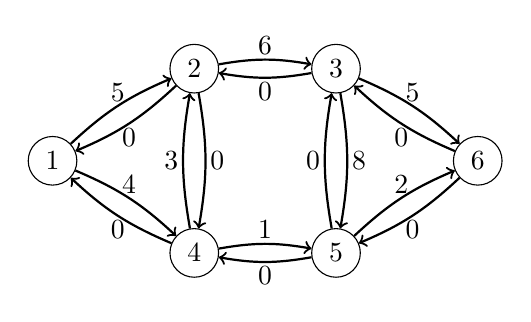
\begin{tikzpicture}[scale=0.9,label distance=-2mm]
\node[draw, circle] (1) at (1,1.3) {$1$};
\node[draw, circle] (2) at (3,2.6) {$2$};
\node[draw, circle] (3) at (5,2.6) {$3$};
\node[draw, circle] (4) at (7,1.3) {$6$};
\node[draw, circle] (5) at (3,0) {$4$};
\node[draw, circle] (6) at (5,0) {$5$};

\path[draw,thick,->] (1) edge [bend left=10] node[font=\small,label=5] {} (2);
\path[draw,thick,->] (2) edge [bend left=10] node[font=\small,label=below:0] {} (1);
\path[draw,thick,->] (2) edge [bend left=10] node[font=\small,label=6] {} (3);
\path[draw,thick,->] (3) edge [bend left=10] node[font=\small,label=below:0] {} (2);
\path[draw,thick,->] (3) edge [bend left=10] node[font=\small,label=5] {} (4);
\path[draw,thick,->] (4) edge [bend left=10] node[font=\small,label=below:0] {} (3);
\path[draw,thick,->] (1) edge [bend left=10] node[font=\small,label=4] {} (5);
\path[draw,thick,->] (5) edge [bend left=10] node[font=\small,label=below:0] {} (1);
\path[draw,thick,->] (5) edge [bend left=10] node[font=\small,label=1] {} (6);
\path[draw,thick,->] (6) edge [bend left=10] node[font=\small,label=below:0] {} (5);
\path[draw,thick,->] (6) edge [bend left=10] node[font=\small,label=2] {} (4);
\path[draw,thick,->] (4) edge [bend left=10] node[font=\small,label=below:0] {} (6);
\path[draw,thick,->] (5) edge [bend left=10] node[font=\small,label=left:3] {} (2);
\path[draw,thick,->] (2) edge [bend left=10] node[font=\small,label=right:0] {} (5);
\path[draw,thick,->] (3) edge [bend left=10] node[font=\small,label=right:8] {} (6);
\path[draw,thick,->] (6) edge [bend left=10] node[font=\small,label=left:0] {} (3);
\end{tikzpicture}
\end{center}
\end{samepage}

\subsubsection{Algoritmin toiminta}

The Ford–Fulkerson algorithm finds at each step
a path from the starting node to the ending node
where each edge has a positive weight.
If there are more than one possible paths,
we can choose any of them.

In the example graph, we can choose, say, the following path:

\begin{center}
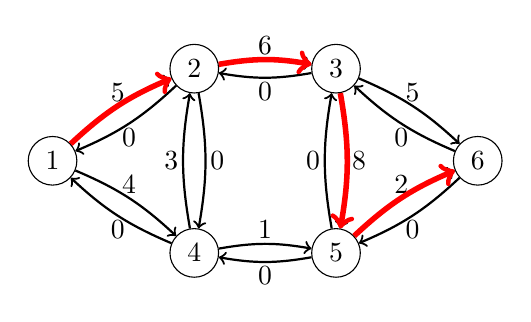
\begin{tikzpicture}[scale=0.9,label distance=-2mm]
\node[draw, circle] (1) at (1,1.3) {$1$};
\node[draw, circle] (2) at (3,2.6) {$2$};
\node[draw, circle] (3) at (5,2.6) {$3$};
\node[draw, circle] (4) at (7,1.3) {$6$};
\node[draw, circle] (5) at (3,0) {$4$};
\node[draw, circle] (6) at (5,0) {$5$};

\path[draw,thick,->] (1) edge [bend left=10] node[font=\small,label=5] {} (2);
\path[draw,thick,->] (2) edge [bend left=10] node[font=\small,label=below:0] {} (1);
\path[draw,thick,->] (2) edge [bend left=10] node[font=\small,label=6] {} (3);
\path[draw,thick,->] (3) edge [bend left=10] node[font=\small,label=below:0] {} (2);
\path[draw,thick,->] (3) edge [bend left=10] node[font=\small,label=5] {} (4);
\path[draw,thick,->] (4) edge [bend left=10] node[font=\small,label=below:0] {} (3);
\path[draw,thick,->] (1) edge [bend left=10] node[font=\small,label=4] {} (5);
\path[draw,thick,->] (5) edge [bend left=10] node[font=\small,label=below:0] {} (1);
\path[draw,thick,->] (5) edge [bend left=10] node[font=\small,label=1] {} (6);
\path[draw,thick,->] (6) edge [bend left=10] node[font=\small,label=below:0] {} (5);
\path[draw,thick,->] (6) edge [bend left=10] node[font=\small,label=2] {} (4);
\path[draw,thick,->] (4) edge [bend left=10] node[font=\small,label=below:0] {} (6);
\path[draw,thick,->] (5) edge [bend left=10] node[font=\small,label=left:3] {} (2);
\path[draw,thick,->] (2) edge [bend left=10] node[font=\small,label=right:0] {} (5);
\path[draw,thick,->] (3) edge [bend left=10] node[font=\small,label=right:8] {} (6);
\path[draw,thick,->] (6) edge [bend left=10] node[font=\small,label=left:0] {} (3);

\path[draw=red,thick,->,line width=2pt] (1) edge [bend left=10] (2);
\path[draw=red,thick,->,line width=2pt] (2) edge [bend left=10] (3);
\path[draw=red,thick,->,line width=2pt] (3) edge [bend left=10] (6);
\path[draw=red,thick,->,line width=2pt] (6) edge [bend left=10] (4);
\end{tikzpicture}
\end{center}

After choosing the path, the flow increases by $x$ units
where $x$ is the smallest weight of an edge in the path.
In addition, the weight of each edge in the path
decreases by $x$, and the weight of each reverse edge
increases by $x$.

In the above path, the weights of the
edges are 5, 6, 8 and 2.
The minimum weight is 2,
so the flow increases by 2
and the new graph is as follows:

\begin{center}
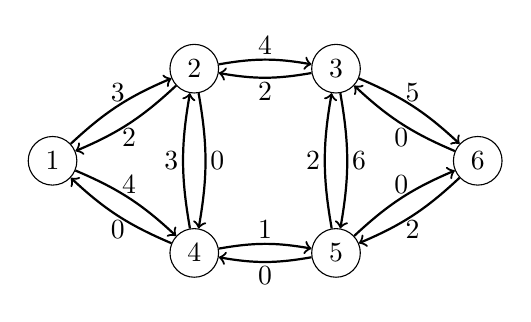
\begin{tikzpicture}[scale=0.9,label distance=-2mm]
\node[draw, circle] (1) at (1,1.3) {$1$};
\node[draw, circle] (2) at (3,2.6) {$2$};
\node[draw, circle] (3) at (5,2.6) {$3$};
\node[draw, circle] (4) at (7,1.3) {$6$};
\node[draw, circle] (5) at (3,0) {$4$};
\node[draw, circle] (6) at (5,0) {$5$};

\path[draw,thick,->] (1) edge [bend left=10] node[font=\small,label=3] {} (2);
\path[draw,thick,->] (2) edge [bend left=10] node[font=\small,label=below:2] {} (1);
\path[draw,thick,->] (2) edge [bend left=10] node[font=\small,label=4] {} (3);
\path[draw,thick,->] (3) edge [bend left=10] node[font=\small,label=below:2] {} (2);
\path[draw,thick,->] (3) edge [bend left=10] node[font=\small,label=5] {} (4);
\path[draw,thick,->] (4) edge [bend left=10] node[font=\small,label=below:0] {} (3);
\path[draw,thick,->] (1) edge [bend left=10] node[font=\small,label=4] {} (5);
\path[draw,thick,->] (5) edge [bend left=10] node[font=\small,label=below:0] {} (1);
\path[draw,thick,->] (5) edge [bend left=10] node[font=\small,label=1] {} (6);
\path[draw,thick,->] (6) edge [bend left=10] node[font=\small,label=below:0] {} (5);
\path[draw,thick,->] (6) edge [bend left=10] node[font=\small,label=0] {} (4);
\path[draw,thick,->] (4) edge [bend left=10] node[font=\small,label=below:2] {} (6);
\path[draw,thick,->] (5) edge [bend left=10] node[font=\small,label=left:3] {} (2);
\path[draw,thick,->] (2) edge [bend left=10] node[font=\small,label=right:0] {} (5);
\path[draw,thick,->] (3) edge [bend left=10] node[font=\small,label=right:6] {} (6);
\path[draw,thick,->] (6) edge [bend left=10] node[font=\small,label=left:2] {} (3);
\end{tikzpicture}
\end{center}

The idea is that increasing the flow decreases the amount of
flow that can go through the edges in the future.
On the other hand, it is possible to adjust the
amount of the flow later
using the reverse edges if it turns out that
we should route the flow in another way.

The algorithm increases the flow as long as
there is a path from the starting node
to the ending node through positive edges.
In the current example, our next path can be as follows:

\begin{center}
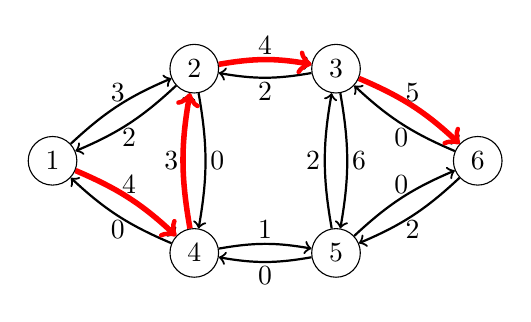
\begin{tikzpicture}[scale=0.9,label distance=-2mm]
\node[draw, circle] (1) at (1,1.3) {$1$};
\node[draw, circle] (2) at (3,2.6) {$2$};
\node[draw, circle] (3) at (5,2.6) {$3$};
\node[draw, circle] (4) at (7,1.3) {$6$};
\node[draw, circle] (5) at (3,0) {$4$};
\node[draw, circle] (6) at (5,0) {$5$};

\path[draw,thick,->] (1) edge [bend left=10] node[font=\small,label=3] {} (2);
\path[draw,thick,->] (2) edge [bend left=10] node[font=\small,label=below:2] {} (1);
\path[draw,thick,->] (2) edge [bend left=10] node[font=\small,label=4] {} (3);
\path[draw,thick,->] (3) edge [bend left=10] node[font=\small,label=below:2] {} (2);
\path[draw,thick,->] (3) edge [bend left=10] node[font=\small,label=5] {} (4);
\path[draw,thick,->] (4) edge [bend left=10] node[font=\small,label=below:0] {} (3);
\path[draw,thick,->] (1) edge [bend left=10] node[font=\small,label=4] {} (5);
\path[draw,thick,->] (5) edge [bend left=10] node[font=\small,label=below:0] {} (1);
\path[draw,thick,->] (5) edge [bend left=10] node[font=\small,label=1] {} (6);
\path[draw,thick,->] (6) edge [bend left=10] node[font=\small,label=below:0] {} (5);
\path[draw,thick,->] (6) edge [bend left=10] node[font=\small,label=0] {} (4);
\path[draw,thick,->] (4) edge [bend left=10] node[font=\small,label=below:2] {} (6);
\path[draw,thick,->] (5) edge [bend left=10] node[font=\small,label=left:3] {} (2);
\path[draw,thick,->] (2) edge [bend left=10] node[font=\small,label=right:0] {} (5);
\path[draw,thick,->] (3) edge [bend left=10] node[font=\small,label=right:6] {} (6);
\path[draw,thick,->] (6) edge [bend left=10] node[font=\small,label=left:2] {} (3);

\path[draw=red,thick,->,line width=2pt] (1) edge [bend left=10] (5);
\path[draw=red,thick,->,line width=2pt] (5) edge [bend left=10] (2);
\path[draw=red,thick,->,line width=2pt] (2) edge [bend left=10] (3);
\path[draw=red,thick,->,line width=2pt] (3) edge [bend left=10] (4);
\end{tikzpicture}
\end{center}

The minimum weight in this path is 3,
so the path increases the flow by 3,
and the total amount of the flow after
processing the path is 5.

\begin{samepage}
The new graph will be as follows:

\begin{center}
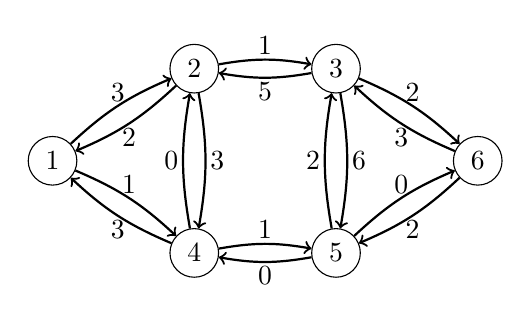
\begin{tikzpicture}[scale=0.9,label distance=-2mm]
\node[draw, circle] (1) at (1,1.3) {$1$};
\node[draw, circle] (2) at (3,2.6) {$2$};
\node[draw, circle] (3) at (5,2.6) {$3$};
\node[draw, circle] (4) at (7,1.3) {$6$};
\node[draw, circle] (5) at (3,0) {$4$};
\node[draw, circle] (6) at (5,0) {$5$};

\path[draw,thick,->] (1) edge [bend left=10] node[font=\small,label=3] {} (2);
\path[draw,thick,->] (2) edge [bend left=10] node[font=\small,label=below:2] {} (1);
\path[draw,thick,->] (2) edge [bend left=10] node[font=\small,label=1] {} (3);
\path[draw,thick,->] (3) edge [bend left=10] node[font=\small,label=below:5] {} (2);
\path[draw,thick,->] (3) edge [bend left=10] node[font=\small,label=2] {} (4);
\path[draw,thick,->] (4) edge [bend left=10] node[font=\small,label=below:3] {} (3);
\path[draw,thick,->] (1) edge [bend left=10] node[font=\small,label=1] {} (5);
\path[draw,thick,->] (5) edge [bend left=10] node[font=\small,label=below:3] {} (1);
\path[draw,thick,->] (5) edge [bend left=10] node[font=\small,label=1] {} (6);
\path[draw,thick,->] (6) edge [bend left=10] node[font=\small,label=below:0] {} (5);
\path[draw,thick,->] (6) edge [bend left=10] node[font=\small,label=0] {} (4);
\path[draw,thick,->] (4) edge [bend left=10] node[font=\small,label=below:2] {} (6);
\path[draw,thick,->] (5) edge [bend left=10] node[font=\small,label=left:0] {} (2);
\path[draw,thick,->] (2) edge [bend left=10] node[font=\small,label=right:3] {} (5);
\path[draw,thick,->] (3) edge [bend left=10] node[font=\small,label=right:6] {} (6);
\path[draw,thick,->] (6) edge [bend left=10] node[font=\small,label=left:2] {} (3);
\end{tikzpicture}
\end{center}
\end{samepage}

We still need two more steps before we have reached a maximum flow.
For example, we can choose the paths
$1 \rightarrow 2 \rightarrow 3 \rightarrow 6$ and
$1 \rightarrow 4 \rightarrow 5 \rightarrow 3 \rightarrow 6$.
Both paths increase the flow by 1,
and the final graph is as follows:

\begin{center}
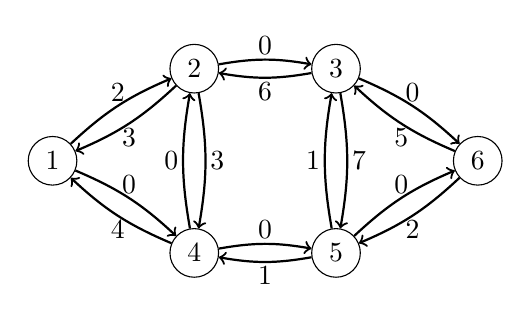
\begin{tikzpicture}[scale=0.9,label distance=-2mm]
\node[draw, circle] (1) at (1,1.3) {$1$};
\node[draw, circle] (2) at (3,2.6) {$2$};
\node[draw, circle] (3) at (5,2.6) {$3$};
\node[draw, circle] (4) at (7,1.3) {$6$};
\node[draw, circle] (5) at (3,0) {$4$};
\node[draw, circle] (6) at (5,0) {$5$};

\path[draw,thick,->] (1) edge [bend left=10] node[font=\small,label=2] {} (2);
\path[draw,thick,->] (2) edge [bend left=10] node[font=\small,label=below:3] {} (1);
\path[draw,thick,->] (2) edge [bend left=10] node[font=\small,label=0] {} (3);
\path[draw,thick,->] (3) edge [bend left=10] node[font=\small,label=below:6] {} (2);
\path[draw,thick,->] (3) edge [bend left=10] node[font=\small,label=0] {} (4);
\path[draw,thick,->] (4) edge [bend left=10] node[font=\small,label=below:5] {} (3);
\path[draw,thick,->] (1) edge [bend left=10] node[font=\small,label=0] {} (5);
\path[draw,thick,->] (5) edge [bend left=10] node[font=\small,label=below:4] {} (1);
\path[draw,thick,->] (5) edge [bend left=10] node[font=\small,label=0] {} (6);
\path[draw,thick,->] (6) edge [bend left=10] node[font=\small,label=below:1] {} (5);
\path[draw,thick,->] (6) edge [bend left=10] node[font=\small,label=0] {} (4);
\path[draw,thick,->] (4) edge [bend left=10] node[font=\small,label=below:2] {} (6);
\path[draw,thick,->] (5) edge [bend left=10] node[font=\small,label=left:0] {} (2);
\path[draw,thick,->] (2) edge [bend left=10] node[font=\small,label=right:3] {} (5);
\path[draw,thick,->] (3) edge [bend left=10] node[font=\small,label=right:7] {} (6);
\path[draw,thick,->] (6) edge [bend left=10] node[font=\small,label=left:1] {} (3);
\end{tikzpicture}
\end{center}

It's not possible to increase the flow anymore,
because there is no path from the starting node
to the ending node with positive edge weights.
Thus, the algorithm terminates and the maximum flow is 7.

\subsubsection{Finding paths}

The Ford–Fulkerson algorithm doesn't specify
how the path that increases the flow should be chosen.
In any case, the algorithm will stop sooner or later
and produce a maximum flow.
However, the efficiency of the algorithm depends on
the way the paths are chosen.

A simple way to find paths is to use depth-first search.
Usually, this works well, but the worst case is that
each path only increases the flow by 1, and the algorithm becomes slow.
Fortunately, we can avoid this by using one of the following
algorithms:

\index{Edmonds–Karp algorithm}

The \key{Edmonds–Karp algorithm}
is an implementation of the
Ford–Fulkerson algorithm where
each path that increases the flow
is chosen so that the number of edges
in the path is minimum.
This can be done by using breadth-first search
instead of depth-first search.
It turns out that this guarantees that
flow increases quickly, and the time complexity
of the algorithm is $O(m^2 n)$.

\index{scaling algorithm}

The \key{scaling algorithm} uses depth-first
search to find paths where the weight of each edge is
at least a minimum value.
Initially, the minimum value is $c$,
the sum of capacities of the edges that
begin at the starting edge.
If the algorithm can't find a path,
the minimum value is divided by 2,
and finally it will be 1.
The time complexity of the algorithm is $O(m^2 \log c)$.

In practice, the scaling algorithm is easier to code
because we can use depth-first search to find paths.
Both algorithms are efficient enough for problems
that typically appear in programming contests.

\subsubsection{Minimum cut}

\index{minimum cut}

It turns out that once the Ford–Fulkerson algorithm
has found a maximum flow,
it has also produced a minimum cut.
Let $A$ be the set of nodes
that can be reached from the starting node
using positive edges.
In the example graph, $A$ contains nodes 1, 2 and 4:

\begin{center}
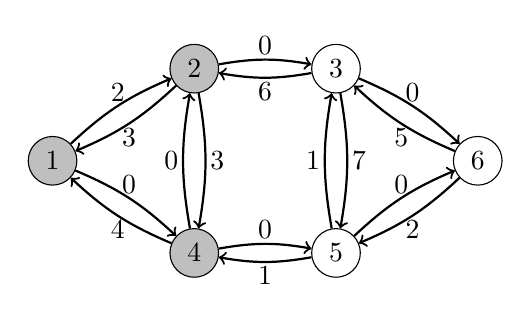
\begin{tikzpicture}[scale=0.9,label distance=-2mm]
\node[draw, circle,fill=lightgray] (1) at (1,1.3) {$1$};
\node[draw, circle,fill=lightgray] (2) at (3,2.6) {$2$};
\node[draw, circle] (3) at (5,2.6) {$3$};
\node[draw, circle] (4) at (7,1.3) {$6$};
\node[draw, circle,fill=lightgray] (5) at (3,0) {$4$};
\node[draw, circle] (6) at (5,0) {$5$};

\path[draw,thick,->] (1) edge [bend left=10] node[font=\small,label=2] {} (2);
\path[draw,thick,->] (2) edge [bend left=10] node[font=\small,label=below:3] {} (1);
\path[draw,thick,->] (2) edge [bend left=10] node[font=\small,label=0] {} (3);
\path[draw,thick,->] (3) edge [bend left=10] node[font=\small,label=below:6] {} (2);
\path[draw,thick,->] (3) edge [bend left=10] node[font=\small,label=0] {} (4);
\path[draw,thick,->] (4) edge [bend left=10] node[font=\small,label=below:5] {} (3);
\path[draw,thick,->] (1) edge [bend left=10] node[font=\small,label=0] {} (5);
\path[draw,thick,->] (5) edge [bend left=10] node[font=\small,label=below:4] {} (1);
\path[draw,thick,->] (5) edge [bend left=10] node[font=\small,label=0] {} (6);
\path[draw,thick,->] (6) edge [bend left=10] node[font=\small,label=below:1] {} (5);
\path[draw,thick,->] (6) edge [bend left=10] node[font=\small,label=0] {} (4);
\path[draw,thick,->] (4) edge [bend left=10] node[font=\small,label=below:2] {} (6);
\path[draw,thick,->] (5) edge [bend left=10] node[font=\small,label=left:0] {} (2);
\path[draw,thick,->] (2) edge [bend left=10] node[font=\small,label=right:3] {} (5);
\path[draw,thick,->] (3) edge [bend left=10] node[font=\small,label=right:7] {} (6);
\path[draw,thick,->] (6) edge [bend left=10] node[font=\small,label=left:1] {} (3);
\end{tikzpicture}
\end{center}

Now the minimum cut consists of the edges in the original graph
that begin at a node in $A$ and end at a node outside $A$,
and whose capacity is fully
used in the maximum flow.
In the above graph, such edges are
$2 \rightarrow 3$ and $4 \rightarrow 5$,
that correspond to the minimum cut $6+1=7$.

Why is the flow produced by the algorithm maximum,
and why is the cut minimum?
The reason for this is that a graph never
contains a flow whose size is larger
than the weight of any cut in the graph.
Hence, always when a flow and a cut are equally large,
they are a maximum flow and a minimum cut.

Let's consider any cut in the graph
where the starting node belongs to set $A$,
the ending node belongs to set $B$
and there are edges between the sets:

\begin{center}
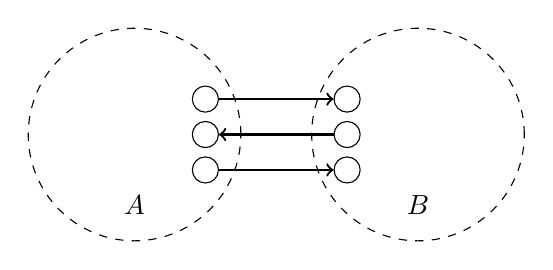
\begin{tikzpicture}[scale=0.9]
\draw[dashed] (-2,0) circle (1.5);
\draw[dashed] (2,0) circle (1.5);

\node at (-2,-1) {$A$};
\node at (2,-1) {$B$};

\node[draw, circle] (1) at (-1,0.5) {};
\node[draw, circle] (2) at (-1,0) {};
\node[draw, circle] (3) at (-1,-0.5) {};
\node[draw, circle] (4) at (1,0.5) {};
\node[draw, circle] (5) at (1,0) {};
\node[draw, circle] (6) at (1,-0.5) {};

\path[draw,thick,->] (1) -- (4);
\path[draw,thick,->] (5) -- (2);
\path[draw,thick,->] (3) -- (6);

\end{tikzpicture}
\end{center}

The weight of the cut is the sum of those edges
that go from set $A$ to set $B$.
This is an upper bound for the amount of flow
in the graph, because the flow has to proceed
from set $A$ to set $B$.
Thus, a maximum flow is smaller than or equal to
any cut in the graph.

On the other hand, the Ford–Fulkerson algorithm
produces a flow that is \emph{exactly} as large
as a cut in the graph.
Thus, the flow has to be a maximum flow,
and the cut has to be a minimum cut.

\section{Rinnakkaiset polut}

Ensimmäisenä virtauslaskennan sovelluksena tarkastelemme
tehtävää, jossa tavoitteena on muodostaa mahdollisimman
monta rinnakkaista polkua verkon alkusolmusta loppusolmuun.
Vaatimuksena on, että jokainen verkon kaari esiintyy
enintään yhdellä polulla.

Esimerkiksi verkossa
\begin{center}
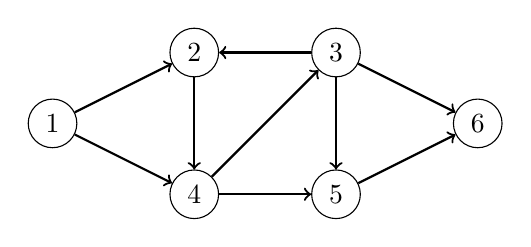
\begin{tikzpicture}[scale=0.9]
\node[draw, circle] (1) at (1,2) {$1$};
\node[draw, circle] (2) at (3,3) {$2$};
\node[draw, circle] (3) at (5,3) {$3$};
\node[draw, circle] (4) at (3,1) {$4$};
\node[draw, circle] (5) at (5,1) {$5$};
\node[draw, circle] (6) at (7,2) {$6$};
\path[draw,thick,->] (1) -- (2);
\path[draw,thick,->] (1) -- (4);
\path[draw,thick,->] (2) -- (4);
\path[draw,thick,->] (3) -- (2);
\path[draw,thick,->] (3) -- (5);
\path[draw,thick,->] (3) -- (6);
\path[draw,thick,->] (4) -- (3);
\path[draw,thick,->] (4) -- (5);
\path[draw,thick,->] (5) -- (6);
\end{tikzpicture}
\end{center}
pystyy muodostamaan kaksi rinnakkaista polkua solmusta 1 solmuun 6.
Tämä toteutuu valitsemalla polut
$1 \rightarrow 2 \rightarrow 4 \rightarrow 3 \rightarrow 6$
ja $1 \rightarrow 4 \rightarrow 5 \rightarrow 6$:

\begin{center}
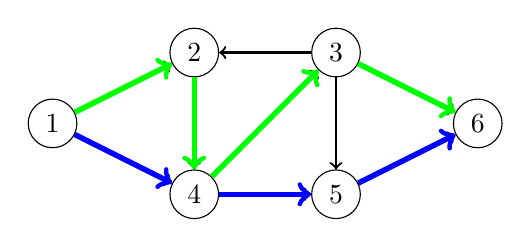
\begin{tikzpicture}[scale=0.9]
\node[draw, circle] (1) at (1,2) {$1$};
\node[draw, circle] (2) at (3,3) {$2$};
\node[draw, circle] (3) at (5,3) {$3$};
\node[draw, circle] (4) at (3,1) {$4$};
\node[draw, circle] (5) at (5,1) {$5$};
\node[draw, circle] (6) at (7,2) {$6$};
\path[draw,thick,->] (1) -- (2);
\path[draw,thick,->] (1) -- (4);
\path[draw,thick,->] (2) -- (4);
\path[draw,thick,->] (3) -- (2);
\path[draw,thick,->] (3) -- (5);
\path[draw,thick,->] (3) -- (6);
\path[draw,thick,->] (4) -- (3);
\path[draw,thick,->] (4) -- (5);
\path[draw,thick,->] (5) -- (6);

\path[draw=green,thick,->,line width=2pt] (1) -- (2);
\path[draw=green,thick,->,line width=2pt] (2) -- (4);
\path[draw=green,thick,->,line width=2pt] (4) -- (3);
\path[draw=green,thick,->,line width=2pt] (3) -- (6);

\path[draw=blue,thick,->,line width=2pt] (1) -- (4);
\path[draw=blue,thick,->,line width=2pt] (4) -- (5);
\path[draw=blue,thick,->,line width=2pt] (5) -- (6);
\end{tikzpicture}
\end{center}

Osoittautuu, että suurin rinnakkaisten polkujen määrä
on yhtä suuri kuin maksimivirtaus verkossa,
jossa jokaisen kaaren kapasiteetti on 1.
Kun maksimivirtaus on muodostettu,
rinnakkaiset polut voi löytää
ahneesti etsimällä alkusolmusta loppusolmuun
kulkevia polkuja.

Tarkastellaan sitten tehtävän muunnelmaa,
jossa jokainen solmu (alku- ja loppusolmua lukuun ottamatta)
saa esiintyä enintään yhdellä polulla.
Tämän rajoituksen seurauksena äskeisessä verkossa
voi muodostaa vain yhden polun,
koska solmu 4 ei voi esiintyä monella polulla:

\begin{center}
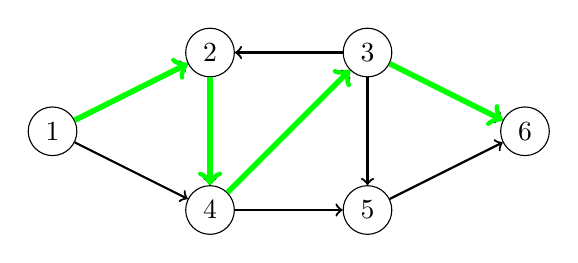
\begin{tikzpicture}
\node[draw, circle] (1) at (1,2) {$1$};
\node[draw, circle] (2) at (3,3) {$2$};
\node[draw, circle] (3) at (5,3) {$3$};
\node[draw, circle] (4) at (3,1) {$4$};
\node[draw, circle] (5) at (5,1) {$5$};
\node[draw, circle] (6) at (7,2) {$6$};
\path[draw,thick,->] (1) -- (2);
\path[draw,thick,->] (1) -- (4);
\path[draw,thick,->] (2) -- (4);
\path[draw,thick,->] (3) -- (2);
\path[draw,thick,->] (3) -- (5);
\path[draw,thick,->] (3) -- (6);
\path[draw,thick,->] (4) -- (3);
\path[draw,thick,->] (4) -- (5);
\path[draw,thick,->] (5) -- (6);

\path[draw=green,thick,->,line width=2pt] (1) -- (2);
\path[draw=green,thick,->,line width=2pt] (2) -- (4);
\path[draw=green,thick,->,line width=2pt] (4) -- (3);
\path[draw=green,thick,->,line width=2pt] (3) -- (6);
\end{tikzpicture}
\end{center}

Tavallinen keino rajoittaa solmun kautta kulkevaa
virtausta on jakaa solmu tulosolmuksi ja lähtösolmuksi.
Kaikki solmuun tulevat kaaret saapuvat tulosolmuun
ja kaikki solmusta lähtevät kaaret poistuvat lähtösolmusta.
Lisäksi tulosolmusta lähtösolmuun on kaari,
jossa on haluttu kapasiteetti.

Tässä tapauksessa verkosta tulee seuraava:
\begin{center}
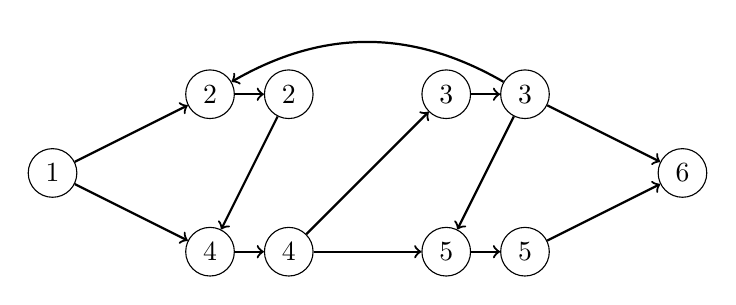
\begin{tikzpicture}
\node[draw, circle] (1) at (1,2) {$1$};

\node[draw, circle] (2a) at (3,3) {$2$};
\node[draw, circle] (3a) at (6,3) {$3$};
\node[draw, circle] (4a) at (3,1) {$4$};
\node[draw, circle] (5a) at (6,1) {$5$};

\node[draw, circle] (2b) at (4,3) {$2$};
\node[draw, circle] (3b) at (7,3) {$3$};
\node[draw, circle] (4b) at (4,1) {$4$};
\node[draw, circle] (5b) at (7,1) {$5$};

\node[draw, circle] (6) at (9,2) {$6$};

\path[draw,thick,->] (2a) -- (2b);
\path[draw,thick,->] (3a) -- (3b);
\path[draw,thick,->] (4a) -- (4b);
\path[draw,thick,->] (5a) -- (5b);

\path[draw,thick,->] (1) -- (2a);
\path[draw,thick,->] (1) -- (4a);
\path[draw,thick,->] (2b) -- (4a);
\path[draw,thick,->] (3b) edge [bend right=30] (2a);
\path[draw,thick,->] (3b) -- (5a);
\path[draw,thick,->] (3b) -- (6);
\path[draw,thick,->] (4b) -- (3a);
\path[draw,thick,->] (4b) -- (5a);
\path[draw,thick,->] (5b) -- (6);
\end{tikzpicture}
\end{center}

Tämän verkon maksimivirtaus on:
\begin{center}
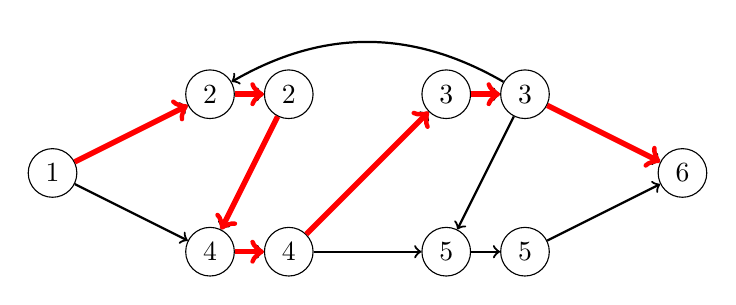
\begin{tikzpicture}
\node[draw, circle] (1) at (1,2) {$1$};

\node[draw, circle] (2a) at (3,3) {$2$};
\node[draw, circle] (3a) at (6,3) {$3$};
\node[draw, circle] (4a) at (3,1) {$4$};
\node[draw, circle] (5a) at (6,1) {$5$};

\node[draw, circle] (2b) at (4,3) {$2$};
\node[draw, circle] (3b) at (7,3) {$3$};
\node[draw, circle] (4b) at (4,1) {$4$};
\node[draw, circle] (5b) at (7,1) {$5$};

\node[draw, circle] (6) at (9,2) {$6$};

\path[draw,thick,->] (2a) -- (2b);
\path[draw,thick,->] (3a) -- (3b);
\path[draw,thick,->] (4a) -- (4b);
\path[draw,thick,->] (5a) -- (5b);

\path[draw,thick,->] (1) -- (2a);
\path[draw,thick,->] (1) -- (4a);
\path[draw,thick,->] (2b) -- (4a);
\path[draw,thick,->] (3b) edge [bend right=30] (2a);
\path[draw,thick,->] (3b) -- (5a);
\path[draw,thick,->] (3b) -- (6);
\path[draw,thick,->] (4b) -- (3a);
\path[draw,thick,->] (4b) -- (5a);
\path[draw,thick,->] (5b) -- (6);

\path[draw=red,thick,->,line width=2pt] (1) -- (2a);
\path[draw=red,thick,->,line width=2pt] (2a) -- (2b);
\path[draw=red,thick,->,line width=2pt] (2b) -- (4a);
\path[draw=red,thick,->,line width=2pt] (4a) -- (4b);
\path[draw=red,thick,->,line width=2pt] (4b) -- (3a);
\path[draw=red,thick,->,line width=2pt] (3a) -- (3b);
\path[draw=red,thick,->,line width=2pt] (3b) -- (6);
\end{tikzpicture}
\end{center}

Tämä tarkoittaa, että verkossa on mahdollista muodostaa
vain yksi polku alkusolmusta lähtösolmuun,
kun sama solmu ei saa esiintyä monessa polussa.

\section{Maksimiparitus}

\index{paritus@paritus}
\index{maksimiparitus@maksimiparitus}

\key{Maksimiparitus} on suurin mahdollinen joukko
verkon solmuista muodostettuja pareja,
jolle pätee,
että jokaisen parin välillä on kaari verkossa
ja jokainen solmu kuuluu enintään yhteen pariin.

Maksimiparituksen etsimiseen yleisessä
verkossa on olemassa polynominen algoritmi,
mutta se on hyvin monimutkainen.
Tässä luvussa keskitymmekin tilanteeseen,
jossa verkko on kaksijakoinen.
Tällöin maksimiparituksen pystyy etsimään
helposti virtauslaskennan avulla.

\subsubsection{Maksimiparituksen etsiminen}

Kaksijakoinen verkko voidaan esittää niin,
että se muodostuu vasemman ja oikean puolen
solmuista ja kaikki verkon kaaret kulkevat puolten välillä.
Tarkastellaan esimerkkinä seuraavaa verkkoa:

\begin{center}
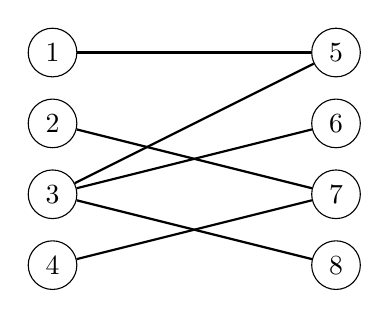
\begin{tikzpicture}[scale=0.60]
\node[draw, circle] (1) at (2,4.5) {1};
\node[draw, circle] (2) at (2,3) {2};
\node[draw, circle] (3) at (2,1.5) {3};
\node[draw, circle] (4) at (2,0) {4};
\node[draw, circle] (5) at (8,4.5) {5};
\node[draw, circle] (6) at (8,3) {6};
\node[draw, circle] (7) at (8,1.5) {7};
\node[draw, circle] (8) at (8,0) {8};

\path[draw,thick,-] (1) -- (5);
\path[draw,thick,-] (2) -- (7);
\path[draw,thick,-] (3) -- (5);
\path[draw,thick,-] (3) -- (6);
\path[draw,thick,-] (3) -- (8);
\path[draw,thick,-] (4) -- (7);
\end{tikzpicture}
\end{center}

Tässä verkossa maksimiparituksen koko on 3:
\begin{center}
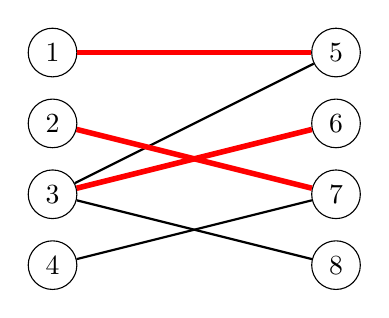
\begin{tikzpicture}[scale=0.60]
\node[draw, circle] (1) at (2,4.5) {1};
\node[draw, circle] (2) at (2,3) {2};
\node[draw, circle] (3) at (2,1.5) {3};
\node[draw, circle] (4) at (2,0) {4};
\node[draw, circle] (5) at (8,4.5) {5};
\node[draw, circle] (6) at (8,3) {6};
\node[draw, circle] (7) at (8,1.5) {7};
\node[draw, circle] (8) at (8,0) {8};

\path[draw,thick,-] (1) -- (5);
\path[draw,thick,-] (2) -- (7);
\path[draw,thick,-] (3) -- (5);
\path[draw,thick,-] (3) -- (6);
\path[draw,thick,-] (3) -- (8);
\path[draw,thick,-] (4) -- (7);

\path[draw=red,thick,-,line width=2pt] (1) -- (5);
\path[draw=red,thick,-,line width=2pt] (2) -- (7);
\path[draw=red,thick,-,line width=2pt] (3) -- (6);
\end{tikzpicture}
\end{center}

Kaksijakoisen verkon maksimiparitus
vastaa maksimivirtausta verkossa,
johon on lisätty alkusolmu ja loppusolmu.
Alkusolmusta on kaari jokaiseen vasemman
puolen solmuun, ja vastaavasti loppusolmuun
on kaari jokaisesta oikean puolen solmusta.
Jokaisen kaaren kapasiteettina on 1.

Esimerkissä tuloksena on seuraava verkko:

\begin{center}
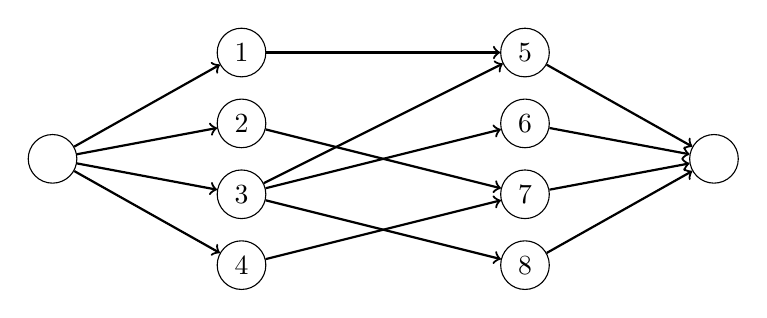
\begin{tikzpicture}[scale=0.60]
\node[draw, circle] (1) at (2,4.5) {1};
\node[draw, circle] (2) at (2,3) {2};
\node[draw, circle] (3) at (2,1.5) {3};
\node[draw, circle] (4) at (2,0) {4};
\node[draw, circle] (5) at (8,4.5) {5};
\node[draw, circle] (6) at (8,3) {6};
\node[draw, circle] (7) at (8,1.5) {7};
\node[draw, circle] (8) at (8,0) {8};

\node[draw, circle] (a) at (-2,2.25) {\phantom{0}};
\node[draw, circle] (b) at (12,2.25) {\phantom{0}};

\path[draw,thick,->] (1) -- (5);
\path[draw,thick,->] (2) -- (7);
\path[draw,thick,->] (3) -- (5);
\path[draw,thick,->] (3) -- (6);
\path[draw,thick,->] (3) -- (8);
\path[draw,thick,->] (4) -- (7);

\path[draw,thick,->] (a) -- (1);
\path[draw,thick,->] (a) -- (2);
\path[draw,thick,->] (a) -- (3);
\path[draw,thick,->] (a) -- (4);
\path[draw,thick,->] (5) -- (b);
\path[draw,thick,->] (6) -- (b);
\path[draw,thick,->] (7) -- (b);
\path[draw,thick,->] (8) -- (b);
\end{tikzpicture}
\end{center}

Tämän verkon maksimivirtaus on yhtä suuri kuin
alkuperäisen verkon maksimiparitus,
koska virtaus muodostuu joukosta polkuja
alkusolmusta loppusolmuun ja jokainen
polku ottaa mukaan uuden kaaren paritukseen.
Tässä tapauksessa maksimivirtaus on 3,
joten maksimiparitus on myös 3.

\subsubsection{Hallin lause}

\index{Hallin lause@Hallin lause}
\index{txydellinen paritus@täydellinen paritus}

\key{Hallin lause} antaa ehdon, milloin kaksijakoiseen
verkkoon voidaan muodostaa paritus,
joka sisältää kaikki toisen puolen solmut.
Jos kummallakin puolella on yhtä monta solmua,
Hallin lause kertoo, voidaanko muodostaa
\key{täydellinen paritus},
jossa kaikki solmut paritetaan keskenään.

Oletetaan, että haluamme muodostaa parituksen,
johon kuuluvat kaikki vasemman puolen solmut.
Olkoon $X$ jokin joukko vasemman puolen solmuja
ja $f(X)$ näiden solmujen naapurien joukko.
Hallin lauseen mukaan paritus on mahdollinen,
kun jokaiselle joukolle $X$
pätee $|X| \le |f(X)|$.

Tarkastellaan Hallin lauseen merkitystä esimerkkiverkossa.
Valitaan ensin $X=\{1,3\}$, jolloin $f(X)=\{5,6,8\}$:

\begin{center}
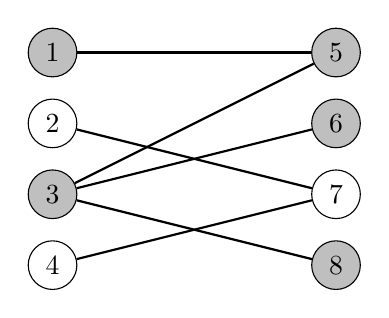
\begin{tikzpicture}[scale=0.60]
\node[draw, circle, fill=lightgray] (1) at (2,4.5) {1};
\node[draw, circle] (2) at (2,3) {2};
\node[draw, circle, fill=lightgray] (3) at (2,1.5) {3};
\node[draw, circle] (4) at (2,0) {4};
\node[draw, circle, fill=lightgray] (5) at (8,4.5) {5};
\node[draw, circle, fill=lightgray] (6) at (8,3) {6};
\node[draw, circle] (7) at (8,1.5) {7};
\node[draw, circle, fill=lightgray] (8) at (8,0) {8};

\path[draw,thick,-] (1) -- (5);
\path[draw,thick,-] (2) -- (7);
\path[draw,thick,-] (3) -- (5);
\path[draw,thick,-] (3) -- (6);
\path[draw,thick,-] (3) -- (8);
\path[draw,thick,-] (4) -- (7);
\end{tikzpicture}
\end{center}

Tämä täyttää Hallin lauseen ehdon, koska $|X|=2$ ja $|f(X)|=3$.
Valitaan sitten $X=\{2,4\}$, jolloin $f(X)=\{7\}$:

\begin{center}
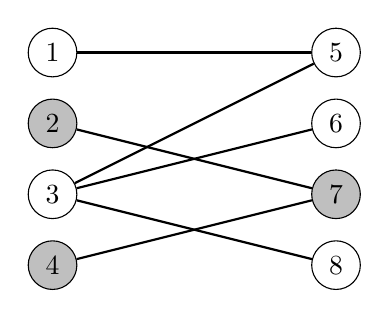
\begin{tikzpicture}[scale=0.60]
\node[draw, circle] (1) at (2,4.5) {1};
\node[draw, circle, fill=lightgray] (2) at (2,3) {2};
\node[draw, circle] (3) at (2,1.5) {3};
\node[draw, circle, fill=lightgray] (4) at (2,0) {4};
\node[draw, circle] (5) at (8,4.5) {5};
\node[draw, circle] (6) at (8,3) {6};
\node[draw, circle, fill=lightgray] (7) at (8,1.5) {7};
\node[draw, circle] (8) at (8,0) {8};

\path[draw,thick,-] (1) -- (5);
\path[draw,thick,-] (2) -- (7);
\path[draw,thick,-] (3) -- (5);
\path[draw,thick,-] (3) -- (6);
\path[draw,thick,-] (3) -- (8);
\path[draw,thick,-] (4) -- (7);
\end{tikzpicture}
\end{center}

Tässä tapauksessa $|X|=2$ ja $|f(X)|=1$, joten Hallin lauseen ehto
ei ole voimassa.
Tämä tarkoittaa, että verkossa
ei ole mahdollista muodostaa täydellistä paritusta,
johon kuuluvat kaikki vasemman puolen solmut.
Tämä on myös odotettu tulos, koska verkon maksimiparitus on 3 eikä 4.

Jos Hallin lauseen ehto ei päde, osajoukko $X$
kertoo syyn sille, miksi paritusta ei voi muodostaa.
Koska $X$ sisältää enemmän solmuja kuin $f(X)$,
kaikille $X$:n solmuille ei riitä paria oikealta.
Esimerkiksi yllä molemmat solmut 2 ja 4 tulisi
yhdistää solmuun 7, mutta tämä ei ole mahdollista.

\subsubsection{Kőnigin lause}

\index{Kőnigin lause}
\index{solmupeite@solmupeite}
\index{pienin solmupeite@pienin solmupeite}

\key{Kőnigin lause} tarjoaa tehokkaan
tavan muodostaa kaksijakoiselle verkolle
\key{pienin solmupeite} eli pienin sellainen
solmujen joukko, että jokaisesta verkon kaaresta ainakin
toinen päätesolmuista kuuluu joukkoon.

Yleisessä verkossa pienimmän solmupeitteen
etsiminen on NP-vaikea ongelma.
Sen sijaan kaksijakoisessa verkossa
Kőnigin lauseen nojalla maksimiparitus ja
pienin solmupeite ovat aina yhtä suuria,
minkä ansiosta
pienimmän solmupeitteen voi
etsiä tehokkaasti virtauslaskennan avulla.

Tarkastellaan taas seuraavaa verkkoa,
jonka maksimiparituksen koko on 3:
\begin{center}
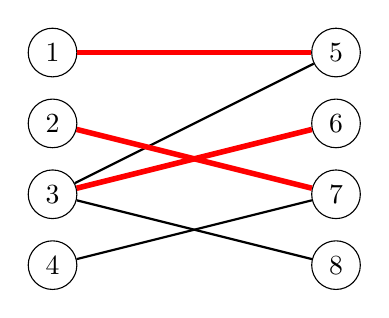
\begin{tikzpicture}[scale=0.60]
\node[draw, circle] (1) at (2,4.5) {1};
\node[draw, circle] (2) at (2,3) {2};
\node[draw, circle] (3) at (2,1.5) {3};
\node[draw, circle] (4) at (2,0) {4};
\node[draw, circle] (5) at (8,4.5) {5};
\node[draw, circle] (6) at (8,3) {6};
\node[draw, circle] (7) at (8,1.5) {7};
\node[draw, circle] (8) at (8,0) {8};

\path[draw,thick,-] (1) -- (5);
\path[draw,thick,-] (2) -- (7);
\path[draw,thick,-] (3) -- (5);
\path[draw,thick,-] (3) -- (6);
\path[draw,thick,-] (3) -- (8);
\path[draw,thick,-] (4) -- (7);

\path[draw=red,thick,-,line width=2pt] (1) -- (5);
\path[draw=red,thick,-,line width=2pt] (2) -- (7);
\path[draw=red,thick,-,line width=2pt] (3) -- (6);
\end{tikzpicture}
\end{center}
Kőnigin lauseen ansiosta tiedämme nyt,
että myös pienimmän solmupeitteen koko on 3.
Solmupeite voidaan muodostaa seuraavasti:

\begin{center}
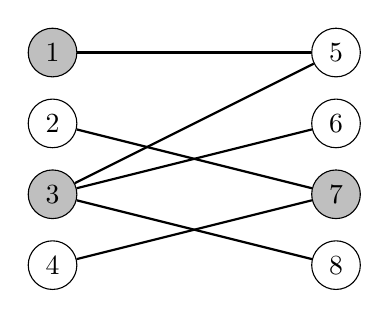
\begin{tikzpicture}[scale=0.60]
\node[draw, circle, fill=lightgray] (1) at (2,4.5) {1};
\node[draw, circle] (2) at (2,3) {2};
\node[draw, circle, fill=lightgray] (3) at (2,1.5) {3};
\node[draw, circle] (4) at (2,0) {4};
\node[draw, circle] (5) at (8,4.5) {5};
\node[draw, circle] (6) at (8,3) {6};
\node[draw, circle, fill=lightgray] (7) at (8,1.5) {7};
\node[draw, circle] (8) at (8,0) {8};

\path[draw,thick,-] (1) -- (5);
\path[draw,thick,-] (2) -- (7);
\path[draw,thick,-] (3) -- (5);
\path[draw,thick,-] (3) -- (6);
\path[draw,thick,-] (3) -- (8);
\path[draw,thick,-] (4) -- (7);
\end{tikzpicture}
\end{center}
Pienin solmupeite muodostuu aina niin,
että jokaisesta maksimiparituksen kaaresta
toinen kaaren päätesolmuista kuuluu peitteeseen.

\index{riippumaton joukko@riippumaton joukko}
\index{suurin riippumaton joukko@suurin riippumaton joukko}

Kun verkosta valitaan kaikki solmut,
jotka \emph{eivät} kuulu pienimpään
solmupeitteeseen, syntyy 
\key{suurin riippumaton joukko}.
Tämä on suurin mahdollinen joukko solmuja,
jossa minkään kahden solmun
välillä ei ole kaarta.
Pienimmän solmupeitteen tavoin
riippumattoman joukon muodostaminen on
NP-vaikea ongelma yleisessä verkossa,
mutta Kőnigin lauseen avulla
ongelma on mahdollista ratkaista
tehokkaasti kaksijakoisessa verkossa.
Esimerkkiverkossa suurin riippumaton joukko on seuraava:

\begin{center}
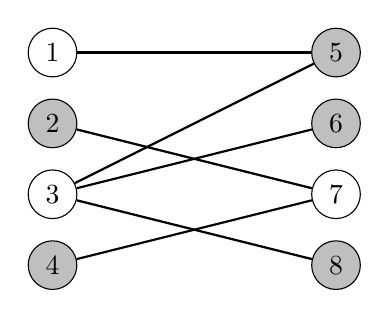
\begin{tikzpicture}[scale=0.60]
\node[draw, circle] (1) at (2,4.5) {1};
\node[draw, circle, fill=lightgray] (2) at (2,3) {2};
\node[draw, circle] (3) at (2,1.5) {3};
\node[draw, circle, fill=lightgray] (4) at (2,0) {4};
\node[draw, circle, fill=lightgray] (5) at (8,4.5) {5};
\node[draw, circle, fill=lightgray] (6) at (8,3) {6};
\node[draw, circle] (7) at (8,1.5) {7};
\node[draw, circle, fill=lightgray] (8) at (8,0) {8};

\path[draw,thick,-] (1) -- (5);
\path[draw,thick,-] (2) -- (7);
\path[draw,thick,-] (3) -- (5);
\path[draw,thick,-] (3) -- (6);
\path[draw,thick,-] (3) -- (8);
\path[draw,thick,-] (4) -- (7);
\end{tikzpicture}
\end{center}

\section{Polkupeitteet}

\index{polkupeite@polkupeite}

\key{Polkupeite} on joukko verkon polkuja,
jotka on valittu niin, että jokainen verkon solmu kuuluu
ainakin yhteen polkuun.
Osoittautuu, että voimme muodostaa
virtauslaskennan avulla
pienimmän polkupeitteen suunnatussa,
syklittömässä verkossa.

Polkupeitteestä on kaksi muunnelmaa:
\key{Solmuerillinen peite} on polkupeite,
jossa jokainen verkon solmu esiintyy tasan yhdessä polussa.
\key{Yleinen peite} taas on polkupeite, jossa sama solmu voi
esiintyä useammassa polussa.
Kummassakin tapauksessa pienin polkupeite löytyy
samanlaisella idealla.

\subsubsection{Solmuerillinen peite}

Tarkastellaan esimerkkinä seuraavaa verkkoa:

\begin{center}
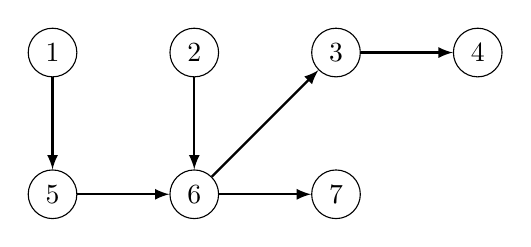
\begin{tikzpicture}[scale=0.9]
\node[draw, circle] (1) at (0,0) {1};
\node[draw, circle] (2) at (2,0) {2};
\node[draw, circle] (3) at (4,0) {3};
\node[draw, circle] (4) at (6,0) {4};
\node[draw, circle] (5) at (0,-2) {5};
\node[draw, circle] (6) at (2,-2) {6};
\node[draw, circle] (7) at (4,-2) {7};

\path[draw,thick,->,>=latex] (1) -- (5);
\path[draw,thick,->,>=latex] (2) -- (6);
\path[draw,thick,->,>=latex] (3) -- (4);
\path[draw,thick,->,>=latex] (5) -- (6);
\path[draw,thick,->,>=latex] (6) -- (3);
\path[draw,thick,->,>=latex] (6) -- (7);
\end{tikzpicture}
\end{center}

Tässä tapauksessa pienin solmuerillinen polkupeite
muodostuu kolmesta polusta.
Voimme valita polut esimerkiksi seuraavasti:

\begin{center}
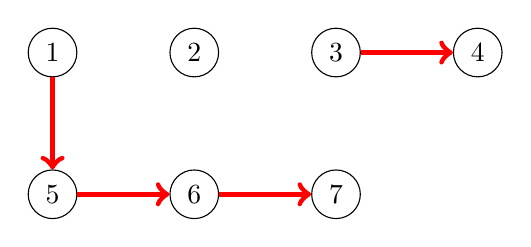
\begin{tikzpicture}[scale=0.9]
\node[draw, circle] (1) at (0,0) {1};
\node[draw, circle] (2) at (2,0) {2};
\node[draw, circle] (3) at (4,0) {3};
\node[draw, circle] (4) at (6,0) {4};
\node[draw, circle] (5) at (0,-2) {5};
\node[draw, circle] (6) at (2,-2) {6};
\node[draw, circle] (7) at (4,-2) {7};

\path[draw=red,thick,->,line width=2pt] (1) -- (5);
\path[draw=red,thick,->,line width=2pt] (5) -- (6);
\path[draw=red,thick,->,line width=2pt] (6) -- (7);
\path[draw=red,thick,->,line width=2pt] (3) -- (4);
\end{tikzpicture}
\end{center}

Huomaa, että yksi poluista sisältää vain solmun 2,
eli on sallittua, että polussa ei ole kaaria.

Polkupeitteen etsiminen voidaan tulkita paritusongelmana
verkossa, jossa jokaista alkuperäisen verkon solmua
vastaa kaksi solmua: vasen ja oikea solmu.
Vasemmasta solmusta oikeaan solmuun on kaari,
jos tällainen kaari esiintyy alkuperäisessä verkossa.
Ideana on, että paritus määrittää, mitkä solmut
ovat yhteydessä toisiinsa poluissa.

Esimerkkiverkossa tilanne on seuraava:

\begin{center}
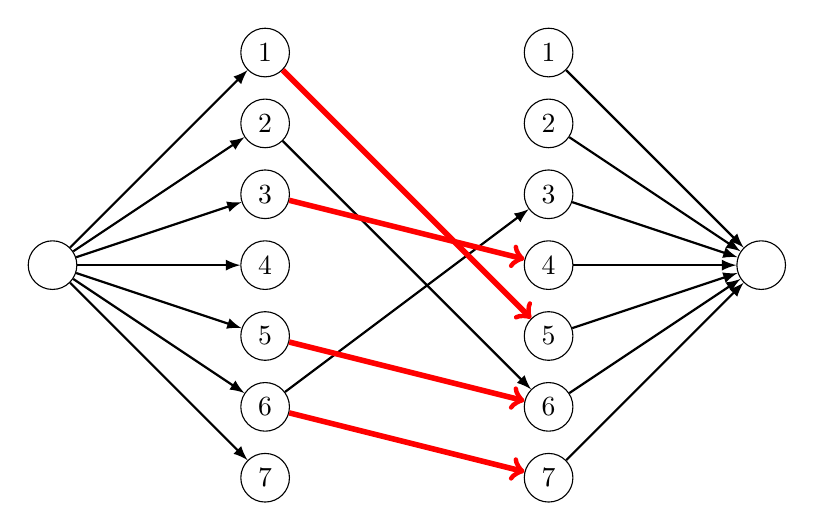
\begin{tikzpicture}[scale=0.9]
\node[draw, circle] (1a) at (0,6) {1};
\node[draw, circle] (2a) at (0,5) {2};
\node[draw, circle] (3a) at (0,4) {3};
\node[draw, circle] (4a) at (0,3) {4};
\node[draw, circle] (5a) at (0,2) {5};
\node[draw, circle] (6a) at (0,1) {6};
\node[draw, circle] (7a) at (0,0) {7};

\node[draw, circle] (1b) at (4,6) {1};
\node[draw, circle] (2b) at (4,5) {2};
\node[draw, circle] (3b) at (4,4) {3};
\node[draw, circle] (4b) at (4,3) {4};
\node[draw, circle] (5b) at (4,2) {5};
\node[draw, circle] (6b) at (4,1) {6};
\node[draw, circle] (7b) at (4,0) {7};

\node[draw, circle] (a) at (-3,3) {\phantom{0}};
\node[draw, circle] (b) at (7,3) {\phantom{0}};

%\path[draw,thick,->,>=latex] (1a) -- (5b);
\path[draw,thick,->,>=latex] (2a) -- (6b);
%\path[draw,thick,->,>=latex] (3a) -- (4b);
%\path[draw,thick,->,>=latex] (5a) -- (6b);
\path[draw,thick,->,>=latex] (6a) -- (3b);
%\path[draw,thick,->,>=latex] (6a) -- (7b);

\path[draw,thick,->,>=latex] (a) -- (1a);
\path[draw,thick,->,>=latex] (a) -- (2a);
\path[draw,thick,->,>=latex] (a) -- (3a);
\path[draw,thick,->,>=latex] (a) -- (4a);
\path[draw,thick,->,>=latex] (a) -- (5a);
\path[draw,thick,->,>=latex] (a) -- (6a);
\path[draw,thick,->,>=latex] (a) -- (7a);

\path[draw,thick,->,>=latex] (1b) -- (b);
\path[draw,thick,->,>=latex] (2b) -- (b);
\path[draw,thick,->,>=latex] (3b) -- (b);
\path[draw,thick,->,>=latex] (4b) -- (b);
\path[draw,thick,->,>=latex] (5b) -- (b);
\path[draw,thick,->,>=latex] (6b) -- (b);
\path[draw,thick,->,>=latex] (7b) -- (b);

\path[draw=red,thick,->,line width=2pt] (1a) -- (5b);
\path[draw=red,thick,->,line width=2pt] (5a) -- (6b);
\path[draw=red,thick,->,line width=2pt] (6a) -- (7b);
\path[draw=red,thick,->,line width=2pt] (3a) -- (4b);

\end{tikzpicture}
\end{center}

Tässä tapauksessa maksimiparitukseen kuuluu neljä kaarta,
jotka vastaavat alkuperäisen verkon kaaria
$1 \rightarrow 5$, $3 \rightarrow 4$,
$5 \rightarrow 6$ ja $6 \rightarrow 7$.
Niinpä pienin solmuerillinen polkupeite syntyy muodostamalla
polut kyseisten kaarten avulla.

Pienimmän polkupeitteen koko on $n-c$, jossa $n$ on verkon
solmujen määrä ja $c$ on maksimiparituksen kaarten määrä.
Esimerkiksi yllä olevassa verkossa pienimmän
polkupeitteen koko on $7-4=3$.

\subsubsection{Yleinen peite}

Yleisessä polkupeitteessä sama solmu voi kuulua moneen polkuun,
minkä ansiosta tarvittava polkujen määrä saattaa olla pienempi.
Esimerkkiverkossa pienin yleinen polkupeite muodostuu
kahdesta polusta seuraavasti:

\begin{center}
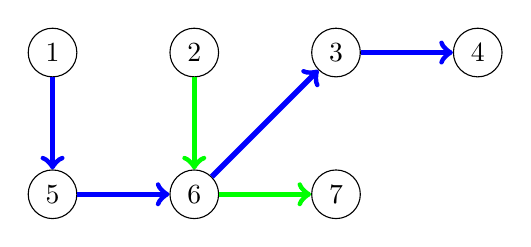
\begin{tikzpicture}[scale=0.9]
\node[draw, circle] (1) at (0,0) {1};
\node[draw, circle] (2) at (2,0) {2};
\node[draw, circle] (3) at (4,0) {3};
\node[draw, circle] (4) at (6,0) {4};
\node[draw, circle] (5) at (0,-2) {5};
\node[draw, circle] (6) at (2,-2) {6};
\node[draw, circle] (7) at (4,-2) {7};

\path[draw=blue,thick,->,line width=2pt] (1) -- (5);
\path[draw=blue,thick,->,line width=2pt] (5) -- (6);
\path[draw=blue,thick,->,line width=2pt] (6) -- (3);
\path[draw=blue,thick,->,line width=2pt] (3) -- (4);
\path[draw=green,thick,->,line width=2pt] (2) -- (6);
\path[draw=green,thick,->,line width=2pt] (6) -- (7);
\end{tikzpicture}
\end{center}

Tässä verkossä yleisessä polkupeitteessä on 2 polkua,
kun taas solmuerillisessä polkupeitteessä on 3 polkua.
Erona on, että yleisessä polkupeitteessä solmua 6
käytetään kahdessa polussa.

Yleisen polkupeitteen voi löytää lähes samalla
tavalla kuin solmuerillisen polkupeitteen.
Riittää täydentää maksimiparituksen verkkoa niin,
että siinä on kaari $a \rightarrow b$ aina silloin,
kun alkuperäisessä verkossa solmusta $a$ pääsee
solmuun $b$ (mahdollisesti usean kaaren kautta).

Nyt esimerkkiverkossa on seuraava tilanne:
\begin{center}
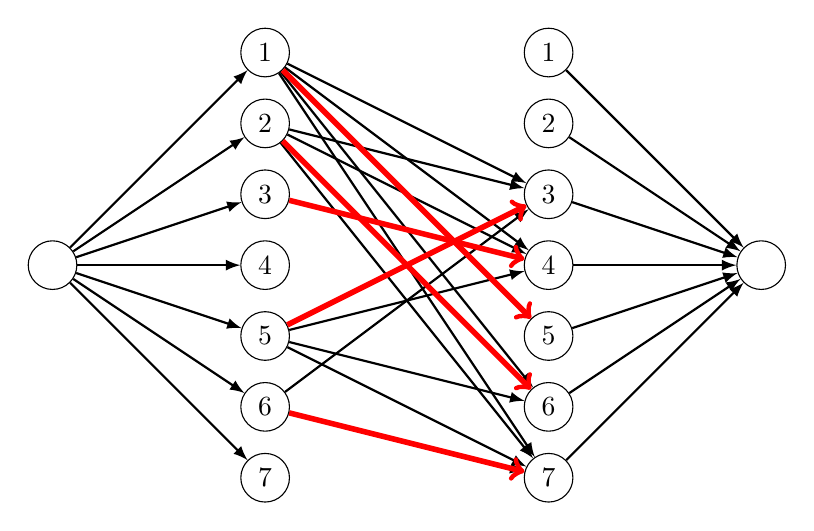
\begin{tikzpicture}[scale=0.9]
\node[draw, circle] (1a) at (0,6) {1};
\node[draw, circle] (2a) at (0,5) {2};
\node[draw, circle] (3a) at (0,4) {3};
\node[draw, circle] (4a) at (0,3) {4};
\node[draw, circle] (5a) at (0,2) {5};
\node[draw, circle] (6a) at (0,1) {6};
\node[draw, circle] (7a) at (0,0) {7};

\node[draw, circle] (1b) at (4,6) {1};
\node[draw, circle] (2b) at (4,5) {2};
\node[draw, circle] (3b) at (4,4) {3};
\node[draw, circle] (4b) at (4,3) {4};
\node[draw, circle] (5b) at (4,2) {5};
\node[draw, circle] (6b) at (4,1) {6};
\node[draw, circle] (7b) at (4,0) {7};

\node[draw, circle] (a) at (-3,3) {\phantom{0}};
\node[draw, circle] (b) at (7,3) {\phantom{0}};


%\path[draw,thick,->,>=latex] (1a) -- (5b);
\path[draw,thick,->,>=latex] (1a) -- (6b);
\path[draw,thick,->,>=latex] (1a) -- (7b);
\path[draw,thick,->,>=latex] (1a) -- (3b);
\path[draw,thick,->,>=latex] (1a) -- (4b);
\path[draw,thick,->,>=latex] (5a) -- (6b);
\path[draw,thick,->,>=latex] (5a) -- (7b);
%\path[draw,thick,->,>=latex] (5a) -- (3b);
\path[draw,thick,->,>=latex] (5a) -- (4b);
\path[draw,thick,->,>=latex] (6a) -- (7b);
%\path[draw,thick,->,>=latex] (6a) -- (7b);
\path[draw,thick,->,>=latex] (6a) -- (3b);
%\path[draw,thick,->,>=latex] (3a) -- (4b);
%\path[draw,thick,->,>=latex] (2a) -- (6b);
\path[draw,thick,->,>=latex] (2a) -- (7b);
\path[draw,thick,->,>=latex] (2a) -- (3b);
\path[draw,thick,->,>=latex] (2a) -- (4b);


\path[draw,thick,->,>=latex] (a) -- (1a);
\path[draw,thick,->,>=latex] (a) -- (2a);
\path[draw,thick,->,>=latex] (a) -- (3a);
\path[draw,thick,->,>=latex] (a) -- (4a);
\path[draw,thick,->,>=latex] (a) -- (5a);
\path[draw,thick,->,>=latex] (a) -- (6a);
\path[draw,thick,->,>=latex] (a) -- (7a);

\path[draw,thick,->,>=latex] (1b) -- (b);
\path[draw,thick,->,>=latex] (2b) -- (b);
\path[draw,thick,->,>=latex] (3b) -- (b);
\path[draw,thick,->,>=latex] (4b) -- (b);
\path[draw,thick,->,>=latex] (5b) -- (b);
\path[draw,thick,->,>=latex] (6b) -- (b);
\path[draw,thick,->,>=latex] (7b) -- (b);

\path[draw=red,thick,->,line width=2pt] (1a) -- (5b);
\path[draw=red,thick,->,line width=2pt] (5a) -- (3b);
\path[draw=red,thick,->,line width=2pt] (3a) -- (4b);
\path[draw=red,thick,->,line width=2pt] (2a) -- (6b);
\path[draw=red,thick,->,line width=2pt] (6a) -- (7b);


% \path[draw=red,thick,->,line width=2pt] (1a) -- (6b);
% \path[draw=red,thick,->,line width=2pt] (1a) -- (7b);
% \path[draw=red,thick,->,line width=2pt] (1a) -- (3b);
% \path[draw=red,thick,->,line width=2pt] (1a) -- (4b);
% \path[draw=red,thick,->,line width=2pt] (5a) -- (6b);
% \path[draw=red,thick,->,line width=2pt] (5a) -- (7b);
% \path[draw=red,thick,->,line width=2pt] (5a) -- (3b);
% \path[draw=red,thick,->,line width=2pt] (5a) -- (4b);
% \path[draw=red,thick,->,line width=2pt] (6a) -- (7b);
% \path[draw=red,thick,->,line width=2pt] (6a) -- (7b);
% \path[draw=red,thick,->,line width=2pt] (6a) -- (3b);
% \path[draw=red,thick,->,line width=2pt] (3a) -- (4b);
% \path[draw=red,thick,->,line width=2pt] (2a) -- (6b);
% \path[draw=red,thick,->,line width=2pt] (2a) -- (7b);
% \path[draw=red,thick,->,line width=2pt] (2a) -- (3b);
% \path[draw=red,thick,->,line width=2pt] (2a) -- (4b);

\end{tikzpicture}
\end{center}


\subsubsection{Dilworthin lause}

\index{Dilworthin lause@Dilworthin lause}
\index{antiketju@antiketju}

\key{Dilworthin lauseen} mukaan suunnatun, syklittömän
verkon pienin yleinen polkupeite
on yhtä suuri kuin suurin verkossa oleva \key{antiketju}
eli kokoelma solmuja,
jossa minkään kahden solmun välillä ei ole polkua.

Esimerkiksi äskeisessä verkossa pienin
yleinen polkupeite sisältää kaksi polkua,
joten verkon suurimmassa antiketjussa on kaksi solmua.
Tällainen antiketju muodostuu esimerkiksi
valitsemalla solmut 3 ja 7:

\begin{center}
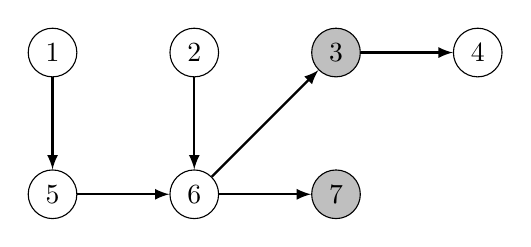
\begin{tikzpicture}[scale=0.9]
\node[draw, circle] (1) at (0,0) {1};
\node[draw, circle] (2) at (2,0) {2};
\node[draw, circle, fill=lightgray] (3) at (4,0) {3};
\node[draw, circle] (4) at (6,0) {4};
\node[draw, circle] (5) at (0,-2) {5};
\node[draw, circle] (6) at (2,-2) {6};
\node[draw, circle, fill=lightgray] (7) at (4,-2) {7};

\path[draw,thick,->,>=latex] (1) -- (5);
\path[draw,thick,->,>=latex] (2) -- (6);
\path[draw,thick,->,>=latex] (3) -- (4);
\path[draw,thick,->,>=latex] (5) -- (6);
\path[draw,thick,->,>=latex] (6) -- (3);
\path[draw,thick,->,>=latex] (6) -- (7);
\end{tikzpicture}
\end{center}

Verkossa ei ole polkua solmusta 3 solmuun 7
eikä polkua solmusta 7 solmuun 3,
joten valinta on kelvollinen.
Toisaalta jos verkosta valitaan mitkä tahansa
kolme solmua, jostain solmusta toiseen on polku.

